\begin{frame}{JRA-3Qとは？}{データ}
  \lead{高さも細かさも足りる再解析は 3 つ。本研究は JRA-3Q}
  {\centering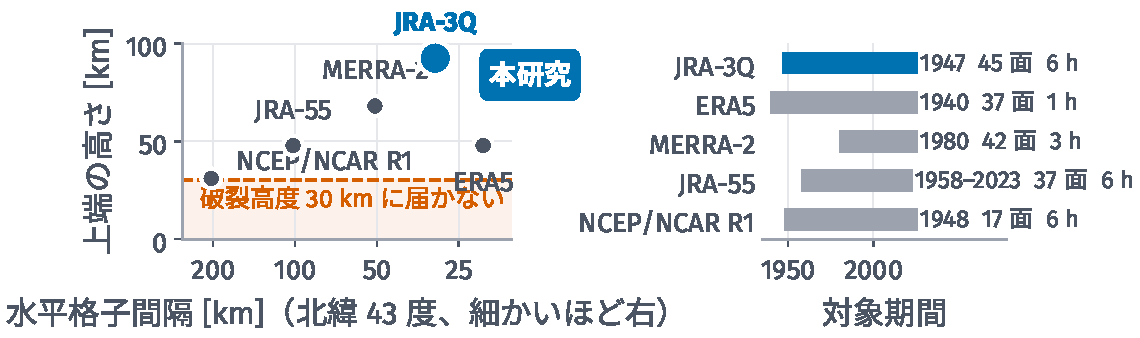
\includegraphics[width=0.92\linewidth,height=104pt,keepaspectratio]{S_reanalyses.pdf}\par}
  \vskip 1mm
  \sub{格子間隔は北緯 43 度での値。JRA-3Q は実測、他は各機関の公表仕様。}
  \srcline{\src{Kalnay+96} \src{Kobayashi+15} \src{Gelaro+17} \src{Hersbach+20}}
\end{frame}
